

\tikzset{every picture/.style={line width=0.75pt}} %set default line width to 0.75pt        

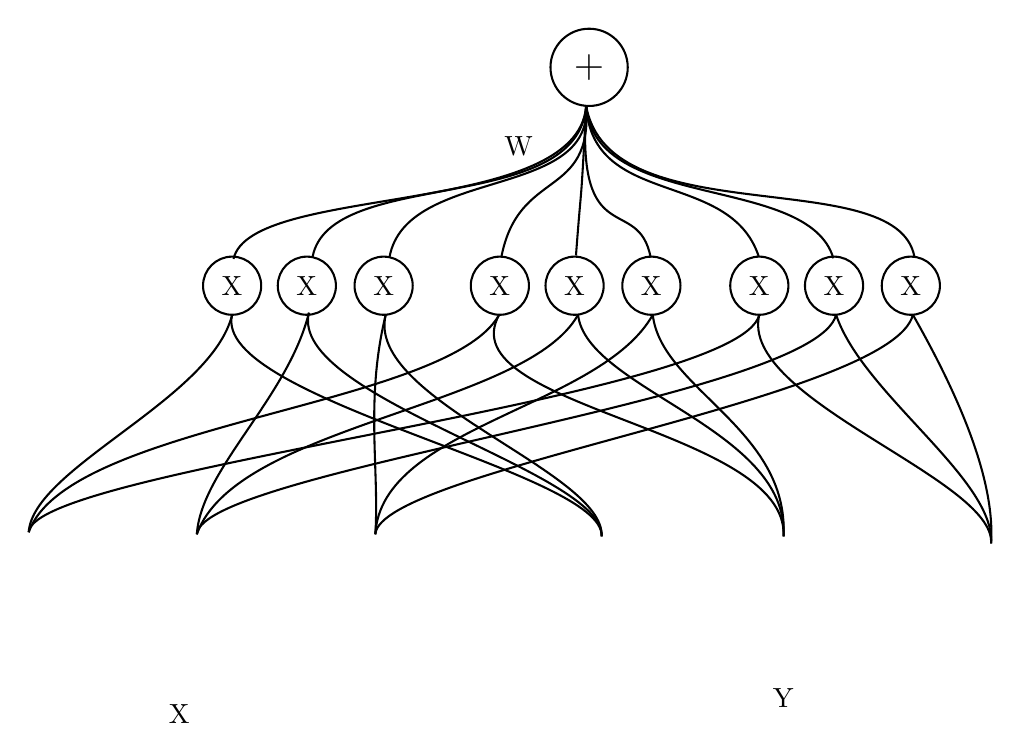
\begin{tikzpicture}[x=0.75pt,y=0.75pt,yscale=-1,xscale=1]
%uncomment if require: \path (0,383); %set diagram left start at 0, and has height of 383

% Plotting does not support converting to Tikz
% Plotting does not support converting to Tikz
% Plotting does not support converting to Tikz
% Plotting does not support converting to Tikz
% Plotting does not support converting to Tikz
% Plotting does not support converting to Tikz
%Curve Lines [id:da947945273944502] 
\draw    (171,177.58) .. controls (161,218.33) and (351,253.33) .. (349,284.33) ;
%Curve Lines [id:da05047724998208092] 
\draw    (171,177.58) .. controls (161,218.33) and (75,251.33) .. (73,282.33) ;
%Curve Lines [id:da03773137720322661] 
\draw    (208,176.58) .. controls (198,217.33) and (156,252.33) .. (154,283.33) ;
%Curve Lines [id:da3244292465400631] 
\draw    (208,176.58) .. controls (198,217.33) and (351,253.33) .. (349,284.33) ;
%Curve Lines [id:da020644663600901003] 
\draw    (245,177.58) .. controls (235,218.33) and (242,252.33) .. (240,283.33) ;
%Curve Lines [id:da5539135653498821] 
\draw    (245,177.58) .. controls (235,218.33) and (351,253.33) .. (349,284.33) ;
%Curve Lines [id:da1374309473218962] 
\draw    (299.67,177.58) .. controls (274.67,222.33) and (91.67,229.33) .. (73,282.33) ;
%Curve Lines [id:da5464682197216861] 
\draw    (299.67,177.58) .. controls (274.67,222.33) and (439.33,232.33) .. (436.67,284.33) ;
%Curve Lines [id:da5210263688647323] 
\draw    (337.67,177.58) .. controls (312.67,222.33) and (172.67,230.33) .. (154,283.33) ;
%Curve Lines [id:da15993872142708243] 
\draw    (337.67,177.58) .. controls (341.67,213.33) and (439.33,232.33) .. (436.67,284.33) ;
%Curve Lines [id:da504697214417569] 
\draw    (373.67,177.58) .. controls (348.67,222.33) and (242.67,231.33) .. (240,283.33) ;
%Curve Lines [id:da056378580674768086] 
\draw    (373.67,177.58) .. controls (377.67,213.33) and (439.33,232.33) .. (436.67,284.33) ;
%Curve Lines [id:da34239451352091654] 
\draw    (425,177.58) .. controls (415,218.33) and (75,251.33) .. (73,282.33) ;
%Curve Lines [id:da5034582933960747] 
\draw    (462,177.58) .. controls (452,218.33) and (156,252.33) .. (154,283.33) ;
%Curve Lines [id:da6784744961144054] 
\draw    (499,177.58) .. controls (489,218.33) and (242,252.33) .. (240,283.33) ;
%Curve Lines [id:da5497330666403395] 
\draw    (425,177.58) .. controls (415,218.33) and (538.67,256.67) .. (536.67,287.67) ;
%Curve Lines [id:da13076459397659135] 
\draw    (462,177.58) .. controls (474.67,215.67) and (538.67,256.67) .. (536.67,287.67) ;
%Curve Lines [id:da11969807748451511] 
\draw    (499,177.58) .. controls (520.67,215.67) and (538.67,256.67) .. (536.67,287.67) ;
%Curve Lines [id:da28989519414938747] 
\draw    (171.67,150.67) .. controls (179.91,114.16) and (337.47,131.26) .. (341.59,77) ;
%Curve Lines [id:da2695278932839822] 
\draw    (209.77,149.68) .. controls (218.01,106.27) and (337.47,130.28) .. (341.59,77) ;
%Curve Lines [id:da20363946739193506] 
\draw    (246.84,149.68) .. controls (255.08,106.27) and (344.68,122.38) .. (341.59,77) ;
%Curve Lines [id:da22681210382350359] 
\draw    (372.67,150) .. controls (366.67,119) and (336.67,148) .. (341.59,77) ;
%Curve Lines [id:da35053652336864016] 
\draw    (300.67,150) .. controls (308.91,106.59) and (344.68,122.38) .. (341.59,77) ;
%Curve Lines [id:da7957569017746662] 
\draw    (336.67,149) .. controls (339.67,109) and (338.67,132) .. (341.59,77) ;
%Curve Lines [id:da2879498014944104] 
\draw    (499.67,149.33) .. controls (490.67,104.33) and (352.67,139.33) .. (341.59,77) ;
%Curve Lines [id:da9077318234949163] 
\draw    (460.67,150.33) .. controls (448.67,109.33) and (345.67,128.33) .. (341.59,77) ;
%Curve Lines [id:da10186900943638544] 
\draw    (424.67,149.33) .. controls (410.67,107.33) and (344.67,126.33) .. (341.59,77) ;

% Text Node
\draw    (171, 163.57) circle [x radius= 14.01, y radius= 14.01]   ;
\draw (171,163.57) node   [align=left] {X};
% Text Node
\draw    (207, 163.57) circle [x radius= 14.01, y radius= 14.01]   ;
\draw (207,163.57) node   [align=left] {X};
% Text Node
\draw    (244, 163.57) circle [x radius= 14.01, y radius= 14.01]   ;
\draw (244,163.57) node   [align=left] {X};
% Text Node
\draw    (343, 58.36) circle [x radius= 18.61, y radius= 18.61]   ;
\draw (343,58.36) node   [align=left] {{\Large +}};
% Text Node
\draw (139,364) node [anchor=north west][inner sep=0.75pt]   [align=left] {X};
% Text Node
\draw (430,356) node [anchor=north west][inner sep=0.75pt]   [align=left] {Y};
% Text Node
\draw    (300, 163.57) circle [x radius= 14.01, y radius= 14.01]   ;
\draw (300,163.57) node   [align=left] {X};
% Text Node
\draw    (336, 163.57) circle [x radius= 14.01, y radius= 14.01]   ;
\draw (336,163.57) node   [align=left] {X};
% Text Node
\draw    (373, 163.57) circle [x radius= 14.01, y radius= 14.01]   ;
\draw (373,163.57) node   [align=left] {X};
% Text Node
\draw    (425, 163.57) circle [x radius= 14.01, y radius= 14.01]   ;
\draw (425,163.57) node   [align=left] {X};
% Text Node
\draw    (461, 163.57) circle [x radius= 14.01, y radius= 14.01]   ;
\draw (461,163.57) node   [align=left] {X};
% Text Node
\draw    (498, 163.57) circle [x radius= 14.01, y radius= 14.01]   ;
\draw (498,163.57) node   [align=left] {X};
% Text Node
\draw (300.67,90) node [anchor=north west][inner sep=0.75pt]   [align=left] {W};


\end{tikzpicture}